\section{Method}
\label{sec:method}

AHE turns harness optimization into a closed loop driven by another agent, with the base model held fixed and only the explicit harness edited.
Our design principle is that every phase of this loop must be \emph{observable}: AHE faithfully records the artifacts each phase produces (the harness components an iteration writes, the rollout trajectories it generates, the edit decisions it commits) and represents them in structured, layered forms that another agent can read and act on.

Three observability layers implement this principle.
\textbf{Component observability} (\S\ref{sec:method:harness}) is realized by a decoupled, file-level harness substrate that maps each failure pattern to a single component class.
\textbf{Experience observability} (\S\ref{sec:method:adb}) is realized by a layered evidence corpus distilled from raw rollouts and indexed for drill-down access.
\textbf{Decision observability} (\S\ref{sec:method:evolve}) is realized by a change manifest that pairs every edit with a self-declared prediction the next round verifies.
The three layers compose into the iteration of Algorithm~\ref{alg:ahe}, which runs unattended round after round.

\subsection{NexAU: an editable, decoupled harness substrate}
\label{sec:method:harness}

\begin{figure}[t]
    \centering
    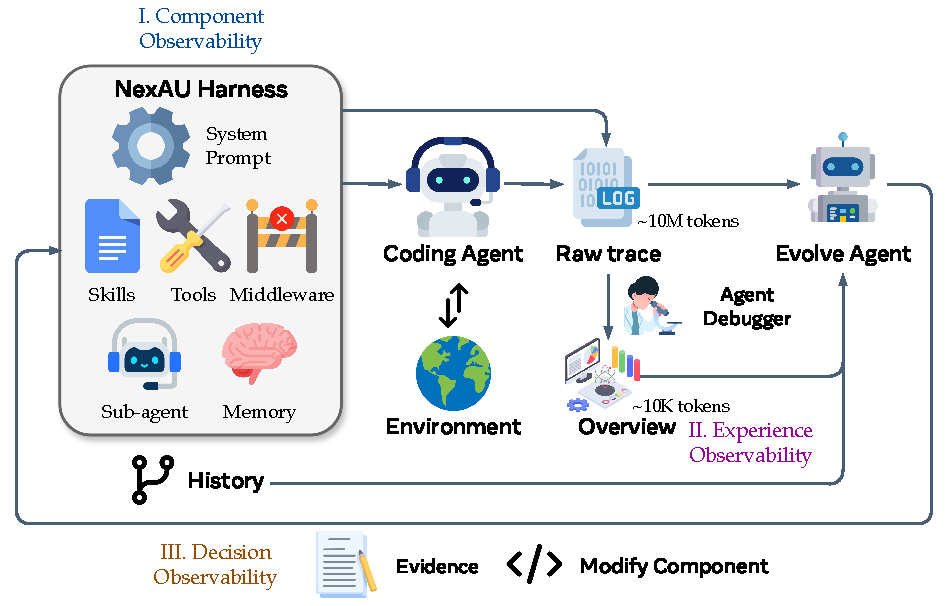
\includegraphics[width=0.8\linewidth]{figures/method.pdf}
    \caption{\textbf{The AHE pipeline links three observable surfaces into one closed loop.} Components, rollout experience, and edit decisions each surface as structured artifacts another agent reads, and every edit becomes a falsifiable prediction the next round verifies.}
    \label{fig:method}
\end{figure}

We instantiate the harness $H$ on the NexAU framework~\citep{nex-agiNexAUAUAgent2025,teamNexN1AgenticModels2025}, which exposes seven orthogonal component types as explicit files at fixed mount points in a single workspace: system prompt, tool description, tool implementation, middleware, skill, sub-agent configuration, and long-term memory.
The component types are loosely coupled, so adding a middleware does not require editing the system prompt, and adding a skill does not require touching any tool.

This decoupling is what realizes \textbf{component observability}: each failure pattern maps to a single component class, giving the evolve agent a clean action space and localizing every pass-rate change to one file rather than scattering it across hundreds of lines of unstructured prompt prose. Each logical edit becomes one commit on the workspace's git history, which yields file-level diffs and rollback granularity for free.

Our seed harness $H_0$ is deliberately minimal: a single shell-execution tool, no middleware, no skills, no sub-agents. A seed already fitted to the target benchmark would contaminate every subsequent edit's attribution, since we could not tell whether a gain came from the loop or from the seed. The minimal seed forces every component AHE adds to earn its place against measured rollouts.


\subsection{Agent Debugger: layered trajectory evidence}
\label{sec:method:adb}

We generate $k$ traces for each task in a benchmark using a harness $H$, which may contain errors resulting from the deficiencies of the harness that can be acted on, but scattered across millions of tokens of raw messages. To extract insights from agent trajectories and enable \textbf{experience observability}, we apply Agent Debugger~\citep{linAgentDebuggerUnderstanding2026} framework to use an agent to explore trajectories framed as a navigable, file-based environment where each trajectory message lives in its own file and is reached through generic shell and scripting tools. Traces with the same query are placed in one environment, and the debugger is required to analyze the root cause of the failure or the success pattern, which is stored in \emph{per-task analysis} report for each task. The analysis also includes pass/fail status of the task to ground the Evolve Agent. Finally, a \emph{benchmark-level overview} is aggregated from every report into a single document as an entry point for every iteration. 

In addition to these reports, we also provide \emph{original} traces in case the agents need to verify the claims in the reports. The traces are provided both in raw form and lightly processed to remove unnecessary content. All of these content is provided as files allowing \textit{progressive disclosure}~\citep{EffectiveContextEngineering} which saves on tokens and enable better agent decisions.


% We use the Agent Debugger~\citep{linAgentDebuggerUnderstanding2026} to convert raw rollout traces into a navigable, file-based corpus in which each trajectory message lives in its own file and is reached through generic shell and scripting tools. This design responds to two pressures of evidence-driven evolution: a single benchmark round emits roughly 10M tokens of raw trace, which would exhaust the editor's context window if served directly, yet arbitrary compression would erase the details on which attribution depends.

% The pipeline distills the traces across four layers separated by information density rather than by compression ratio.
% \ding{182}~The \emph{raw} layer stores every trace verbatim; it is the ground truth against which any higher-level claim can be verified, and the editor reaches it only when a downstream report itself becomes suspect.
% \ding{183}~A \emph{cleaning} layer strips base64 blobs and deduplicates verbatim tool outputs while preserving message order and call structure, removing token noise without distorting causal flow, so downstream analyzers operate on a faithful skeleton at a fraction of the size.
% \ding{184}~A \emph{per-task analysis} layer produces one focused report per task, whose template adapts to the pass/fail signature of the $k$ rollouts (root cause, success pattern, or partial-pass diff); the evolve agent reads it to ground each task-level finding.
% \ding{185}~A \emph{benchmark-wide overview} of roughly 10K tokens aggregates every per-task report into a single document; it is the entry point for every iteration and indexes the rest of the corpus.

% This four-layer pipeline is what realizes \textbf{experience observability}: the rollout history becomes an indexed corpus rather than a summary, where the editor reads the overview first, drills down to a per-task report when a finding needs grounding, and reaches the raw trace only when the report itself is in question. \textit{Progressive disclosure}~\citep{EffectiveContextEngineering} replaces lossy compression.





% \subsection{Evidence-Driven Harness Modification}
% \label{sec:method:evolve}

% The evolution agent reads the analysis layer of \S\ref{sec:method:adb}, edits the workspace of \S\ref{sec:method:harness}, and is bound by three hard constraints that make its own behavior auditable in the next round.

% \paragraph{Constraint 1: Controllability.}
% The evolution agent may write only inside the harness workspace. The runs directory, tracer, verifier, and LLM configuration are read-only, and the framework marks the seed system prompt as non-deletable. These restrictions block the most common shortcuts an unconstrained self-modifier would take, such as disabling the verifier, swapping the model, or raising the reasoning budget, and keep every recorded gain attributable to harness edits.

% \paragraph{Constraint 2: Evidence-driven changes with a recorded prediction.}
% Each edit ships with a manifest entry recorded for that iteration. The entry names the failure evidence behind it, namely which tasks failed and how, the inferred root cause, the targeted fix actually applied, and a predicted impact comprising the tasks the edit is expected to fix together with those it might regress. The manifest is the loop's evidence ledger. In the next round, the loop intersects the predicted-fix and predicted-regression sets with the observed task-level deltas to produce a per-edit verdict. Each edit thereby becomes falsifiable by the next evaluation, which replaces rationale-driven self-justification with a measurable contract between rounds. The same ledger is the data source for the self-assessment analysis in \S\ref{sec:experiments:rq3b}.



\subsection{Evolve Agent: evidence-driven, auditable edits}
\label{sec:method:evolve}

The Evolve Agent closes the AHE loop. In each round it reads the layered evidence corpus produced by the Agent Debugger, decides which harness components to add, modify, or remove, applies those edits to the workspace, and records the reasoning behind every edit. Two constraints govern these edits, and together they realize \textbf{decision observability}: every edit becomes a falsifiable, file-level claim recorded in a versioned manifest, and the next round's verdict either confirms or reverts it.

The first constraint is \textit{controllability}: the Evolve Agent writes only inside the harness workspace, while the runs directory, tracer, verifier, and LLM configuration are read-only, and the seed system prompt (Appendix~\ref{app:prompts:code-seed}) is marked non-deletable.
These restrictions block the shortcuts an unconstrained self-modifier would take, such as disabling the verifier, swapping the model, or raising the reasoning budget, and keep every recorded gain attributable to harness edits.

The second constraint is that every change is \textit{evidence-driven} and ships with a recorded prediction.
Each edit attaches a manifest entry that names the failure evidence, the inferred root cause, the targeted fix, and a predicted impact comprising both expected fixes and at-risk regressions; this manifest is the loop's evidence ledger (see Appendix~\ref{app:prompts:evolve}).
In the next round, the loop intersects the predicted-fix and predicted-regression sets with the observed task-level deltas to produce a per-edit verdict.
Each edit thereby becomes falsifiable by the next evaluation, which replaces rationale-driven self-justification with a measurable contract between rounds.

% Algorithm~\ref{alg:ahe} ties the three substrates into one iteration: rollout, clean, attribute the prior manifest and revert rejected edits, distill, edit, commit. Two design choices are worth noting. We run $k\geq 2$ rollouts per task, so each task carries a pass-rate signal rather than a single binary outcome, which both stabilizes pass@1 against rollout variance and lets partial-pass tasks anchor comparative diagnosis. Attribution runs \emph{before} distillation, so its verdict prunes the harness entering the editor and lands inside the evidence corpus, turning each prior manifest entry into a binding contract rather than an unverified rationale. A one-shot explore agent (Appendix~\ref{app:prompts:explore}) runs once in parallel with iteration~$1$, reading the NexAU source tree together with a curated set of public coding-agent design references to seed a small number of reusable skills; these skills receive no special protection, and from iteration~$2$ onward all edits flow through the Evolve Agent, which may keep, refine, or remove them on the strength of observed rollouts.



% \subsection{Outer Loop}
% \label{sec:method:loop}

% An AHE run begins with a one-shot initialization that primes the workspace with reusable skills, then enters $N$ identical six-phase iterations over the artifacts of \S\S\ref{sec:method:harness}--\ref{sec:method:evolve}. Initialization comes first because it determines what the loop reads in iteration~$1$; the iteration itself is then kept deliberately short, so that the framework can replay any round from the artifacts archived for it.

% \paragraph{Initialization via an explore agent.}
% The seed harness $H_0$ of \S\ref{sec:method:harness} carries no skills and no middleware, only a single shell tool and the seed system prompt. An iteration~$1$ launched directly from this bare $H_0$ would spend most of its evidence budget on framework discovery rather than on diagnosing model failures, and the iteration~$2$ manifest would inherit that cold start. To avoid it, an explore agent runs once in parallel with iteration~$1$ rollouts: it reads the NexAU source tree together with a curated set of public coding-agent design references, then writes a small number of reusable skill files into the workspace under the controllability constraint of \S\ref{sec:method:evolve}. These skills receive no special protection. The evolution agent at iteration~$2$ may keep, refine, or remove any of them on the strength of observed rollouts, and from that round onward all further edits to $H$ flow through Algorithm~\ref{alg:ahe}.

% \paragraph{Six-phase iteration.}
% Algorithm~\ref{alg:ahe} lays out the six phases driven by the evolution agent of \S\ref{sec:method:evolve}; we walk through them below. Phase~1 runs $k$ rollouts of $(M, H_{t-1})$ on every task in $D$, producing the trajectory pool $T_t$. We use $k\geq 2$ so that each task carries a pass-rate signal rather than a single binary outcome, which both stabilizes pass@1 estimates against rollout variance and lets phase~3 attribute task-level deltas with comparative evidence. Phase~2 cleans $T_t$ into $\widetilde{T}_t$ by stripping base64 blobs and deduplicating verbatim tool outputs, keeping message order and call structure intact. Phase~3 runs from iteration~$2$ onward: it intersects the predicted-fix and predicted-regression sets in the prior manifest $C_{t-1}$ with task-level deltas between $T_{t-1}$ and $T_t$ to yield a per-edit verdict $V_t$, after which the rollback rule of \S\ref{sec:method:evolve} reverts every ineffective edit at file granularity. Phase~4 hands $\widetilde{T}_t$ to the Agent Debugger and produces the layered corpus $R_t$ of \S\ref{sec:method:adb}. Phase~5 gives $R_t$ together with $V_t$ to the evolution agent, which writes new components into $H_t$ and records the matching manifest $C_t$ under the three constraints of \S\ref{sec:method:evolve}. Phase~6 commits $H_t$ and $C_t$ as a single git-tagged checkpoint, so any later round can replay or revert it. Placing phase~3 before phase~4 is deliberate: its verdict prunes the baseline $H_{t-1}$ entering phase~5 and lands inside $R_t$ as evidence the evolution agent must reckon with, turning each prior manifest entry into a binding contract across iterations rather than an unverified rationale. The iteration ends by promoting $H_t$ to $H_{\text{best}}$ whenever its pass@1 strictly exceeds the running best.



\begin{algorithm}[htbp]
\caption{AHE outer loop.}
\label{alg:ahe}
\begin{algorithmic}[1]
\Require seed harness $H_0$, base model $M$, benchmark $D$, rollouts per task $k$, max iterations $N$
\State $H_{\text{best}} \gets H_0$
\For{$t = 1$ to $N$}
    \State $T_t \gets \textsc{Rollout}(M, H_{t-1}, D, k)$ \Comment{phase 1: $k$ rollouts per task}
    \State $\widetilde{T}_t \gets \textsc{Clean}(T_t)$ \Comment{phase 2: normalize traces into canonical form}
    \If{$t \geq 2$} \Comment{phase 3: attribute prior manifest, then rollback}
        \State $V_t \gets \textsc{Attribute}(C_{t-1}, T_{t-1}, T_t)$
        \State $H_{t-1} \gets \textsc{Rollback}(H_{t-1}, V_t)$
    \Else
        \State $V_t \gets \emptyset$
    \EndIf
    \State $R_t \gets \textsc{AgentDebugger}(\widetilde{T}_t)$ \Comment{phase 4: layered distillation}
    \State $(H_t, C_t) \gets \textsc{Evolve}(H_{t-1}, R_t, V_t)$ \Comment{phase 5: workspace edits + new manifest}
    \State $\textsc{Commit}(H_t, C_t, t)$ \Comment{phase 6: tag iteration in git}
    \If{$\textsc{Pass@1}(T_t) > \textsc{Pass@1}(H_{\text{best}})$} $H_{\text{best}} \gets H_t$ \EndIf
\EndFor
\State \Return $H_{\text{best}}$
\end{algorithmic}
\end{algorithm}

Algorithm~\ref{alg:ahe} composes the three substrates into one iteration: rollout, clean, attribute the prior manifest and revert rejected edits, distill, edit, commit.
We run $k\geq 2$ rollouts per task so each task carries a pass-rate signal, which stabilizes pass@1 and lets partial-pass tasks anchor comparative diagnosis.
Attribution runs \emph{before} distillation, so its verdict lands inside the evidence corpus and binds each prior manifest entry as a contract rather than a rationale.
A one-shot explore agent (Appendix~\ref{app:prompts:explore}) runs in parallel with iteration~$1$ to seed a small number of reusable skills from the NexAU source and public coding-agent references.
These skills receive no special protection: from iteration~$2$ onward the Evolve Agent may keep, refine, or remove them based on observed rollouts.